\section{A paired extension of segment tests}\label{sec:paired}

The renorming obstruction is proved. To establish midpoint convexity,
we now show that a symmetric pair must grow when its center and
displacement occupy a finite ancestral set and its complement. The
squared-norm form will also be the input for the diamond argument.

\begin{lemma}\label{lem:paired}
Let $H\subset\mathcal F$ be finite and ancestral. If $x,y\in X$
satisfy $x=P_Hx$ and $y=Q_Hy$, then
\begin{equation}\label{eq:paired}
 \frac{\|x+y\|+\|x-y\|}{2}
 \ge\sqrt{\|x\|^2+\|y\|^2/12}.
\end{equation}
More generally, for all $s,t>0$,
\begin{equation}\label{eq:paired-two-parameters}
 \frac{\|x+ty\|+\|x-ty\|}{2}
 \ge\frac{\|x\|+st\|y\|}{\sqrt{1+12s^2}}.
\end{equation}
\end{lemma}

\begin{proof}
We first prove, for every $s>0$,
\begin{equation}\label{eq:paired-parameter}
 \frac{\|x+y\|+\|x-y\|}{2}
 \ge\frac{\|x\|+s\|y\|}{\sqrt{1+12s^2}}.
\end{equation}
Suppose initially that $y$ has finite support. Choose finite tests
$f,k\in J$, supported in $H$ and its complement respectively, with
$\rho(f),\rho(k)\le1$ and pairings as close as desired to $\|x\|$ and
$\|y\|$. The naive tests $f+sk$ and $f-sk$ can have large positive crossing
terms. We will add the same vector to both tail tests; its contribution
to the endpoint average will cancel. To control its size, at each gate
$g$ put
\[
 m_g=\sup_{w\succeq g}|k([g,w])|.
\]
Only finitely many $m_g$ are nonzero, and $\sum_gm_g^2\le1$:
choose an almost maximizing initial segment in each of finitely many
distinct cones and use their disjointness.

For a gate with parent $v\in H$, consider the suffixes $[a,v]$ whose
$f$-sum has magnitude at least $2sm_g$. If $m_g>0$ and such suffixes
exist, choose the shortest one and let $\sigma_g$ be opposite to the
sign of its sum. In all other cases put $\sigma_g=1$. Set
\[
 c=\sum_g\sigma_gm_ge_g,\qquad v^+=c+k,\qquad v^-=c-k.
\]
The gates form an antichain, so $\rho(c)\le1$ and $\rho(v^\pm)\le2$.
Every initial segment in the cone of $g$ has $v^\pm$-sum of sign
$\sigma_g$ or zero, and magnitude at most $2m_g$.

We claim $\rho(f+sv^\pm)^2\le1+12s^2$. Fix a disjoint family of
segments and denote their $f$- and $v^\pm$-sums by $\alpha_i$ and
$\beta_i$. We have $\sum_i\beta_i^2\le4$. A positive cross term
$\alpha_i\beta_i$ can occur only at a crossing segment, with some
gate $g$; different crossing segments use different gates. If
$|\alpha_i|\le2sm_g$, then $2s\alpha_i\beta_i\le8s^2m_g^2$.
Otherwise the head itself reaches the threshold, so it contains the
shortest selected suffix. Write $\alpha'_i$ for that suffix's $f$-sum.
Since $\alpha_i\beta_i>0$ and $\beta_i$ has sign $\sigma_g$, the choice
of $\sigma_g$ gives $\alpha_i\alpha'_i<0$. Thus the selected suffix is
proper, and $|\alpha'_i|\ge2sm_g$ by its selection.
Splitting it off the head increases the sum of squared $f$-sums by
\[
 (\alpha_i-\alpha'_i)^2+(\alpha'_i)^2-\alpha_i^2
 =2(\alpha'_i)^2+2|\alpha_i\alpha'_i|
 \ge4s|\alpha_i|m_g\ge2s\alpha_i\beta_i.
\]
Figure~\ref{fig:paired-cut} shows the proper suffix and the cut,
with the segment index suppressed.
\begin{figure}[tb]
\centering
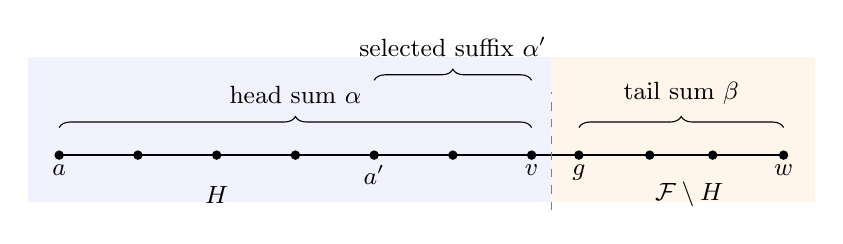
\begin{tikzpicture}[x=1cm,y=1cm,font=\small]
 \fill[blue!5] (-.4,-.6) rectangle (6.25,1.25);
 \fill[orange!8] (6.25,-.6) rectangle (9.6,1.25);
 \draw[thick] (0,0)--(9.2,0);
 \draw[dashed,gray] (6.25,-.7)--(6.25,.8);
 \foreach \x in {0,1,2,3,4,5,6,6.6,7.5,8.3,9.2}
   \fill (\x,0) circle (1.7pt);
 \node[below] at (0,0) {$a$};
 \node[below] at (4,0) {$a'$};
 \node[below] at (6,0) {$v$};
 \node[below] at (6.6,0) {$g$};
 \node[below] at (9.2,0) {$w$};
 \draw[decorate,decoration={brace,amplitude=4pt}] (0,.35)--(6,.35)
   node[midway,above=5pt] {head sum $\alpha$};
 \draw[decorate,decoration={brace,amplitude=4pt}] (4,.95)--(6,.95)
   node[midway,above=5pt] {selected suffix $\alpha'$};
 \draw[decorate,decoration={brace,amplitude=4pt}] (6.6,.35)--(9.2,.35)
   node[midway,above=5pt] {tail sum $\beta$};
 \node at (2,-.5) {$H$};
 \node at (8,-.5) {$\mathcal F\setminus H$};
\end{tikzpicture}
\caption{The threshold cut for a crossing segment. Its head has
$f$-sum $\alpha$ and its selected suffix has $f$-sum $\alpha'$.
When $\alpha\beta>0$ and $|\alpha|>2sm_g$, the sign choice gives
$\alpha\alpha'<0$ and $|\alpha'|\ge2sm_g$.
Cutting immediately before $a'$ therefore increases the squared
$f$-test by at least $2s\alpha\beta$. The vertex spacing is schematic.}
\label{fig:paired-cut}
\end{figure}


These splits involve distinct original segments, so all can be made
simultaneously. Their pieces and the remaining heads are still
disjoint. Thus $\sum_i\alpha_i^2$ together with all the large
positive cross terms is at most $\rho(f)^2\le1$. The small cross terms
cost at most $8s^2$, and the pure tail terms cost at most $4s^2$.
We have controlled both corrected tests. It remains to use them
together so that their common correction disappears.

Test $x+y$ against $(f+sv^+)/\sqrt{1+12s^2}$ and $x-y$ against
$(f+sv^-)/\sqrt{1+12s^2}$. The mixed support terms vanish, and the
two evaluations involving $c$ cancel in the average. Letting the
norming errors tend to zero proves \eqref{eq:paired-parameter}. Finite tails are dense in
$Q_HX$, so \eqref{eq:paired-parameter} holds for every $y=Q_Hy$. If $\|x\|>0$, maximize
its right side by taking $s=\|y\|/(12\|x\|)$; zero values follow
by a limit. The maximum is the right side of \eqref{eq:paired}. Replacing $y$ by $ty$ in \eqref{eq:paired-parameter} proves
\eqref{eq:paired-two-parameters}.
\end{proof}

\begin{proof}[Proof of the midpoint assertion in Theorem~\ref{thm:main}]
For a unit $x\in X$, choose $H$ with $\|x-P_Hx\|<\eta$. For
every unit $y\in\ker P_H$, Lemma~\ref{lem:paired} applied to $P_Hx$ and $ty$ gives
\[
 \frac{\|x+ty\|+\|x-ty\|}{2}
 \ge\sqrt{(1-\eta)^2+t^2/12}-\eta
 \qquad(0<\eta<1).
\]
Take the infimum over these $y$, the supremum over finite-codimensional
subspaces, and let $\eta\downarrow0$. This proves
the asserted bound, since it is independent of the unit center $x$.
\end{proof}
